\chapter{Configuration}
\label{chap-user}

\renewcommand{\headrulewidth}{0.3pt}
\fancyhead[LE]{\thepage} \fancyhead[RE]{\nouppercase{\textbf{\leftmark}}}
\fancyhead[RO]{\thepage} \fancyhead[LO]{\nouppercase{\textbf{\rightmark}}}
\fancyfoot[L,C,R]{}

\setlength{\parindent}{0.35cm}

\minitoc
\newpage
% ================================================================

\section{Généralités}
\label{sec-generalites}

L'extension \cwv~intègre plusieurs fonctionnalités accessibles depuis sa boîte de dialogue d'accueil (\cref{fig-cwv_home_page}) :
\begin{itemize}
    \item une entrée dédiée à la configuration de l'application \cawaqs~(\gui{Settings}
        - \cref{sec_config} à \ref{sec-json_config_project}) ;

    \item des outils d'aide au calage (\gui{Calibration tools} - \cref{sec-calib-tools})
        ;

    \item des fonctionnalités de visualisation des chroniques temporelles de débits et de piézométrie simulées et observées (\gui{Compare Sim/Obs} - \cref{sec-com-simobs})
        ;

    \item des outils de visualisation de la distribution spatiale des composantes hydrologiques (\gui{Spatial Maps} - \cref{sec-spatial-map}) ;

    \item une fonction de visualisation du bilan hydrologique (\gui{Budget Bar Plot}
        - \cref{sec-bufget-barplot}) ;

    \item un visualiseur de régime hydrologique (\gui{Hydrological regime} - \cref{sec-regime-hydro}).
\end{itemize}

\begin{figure}[H]
    \centering
    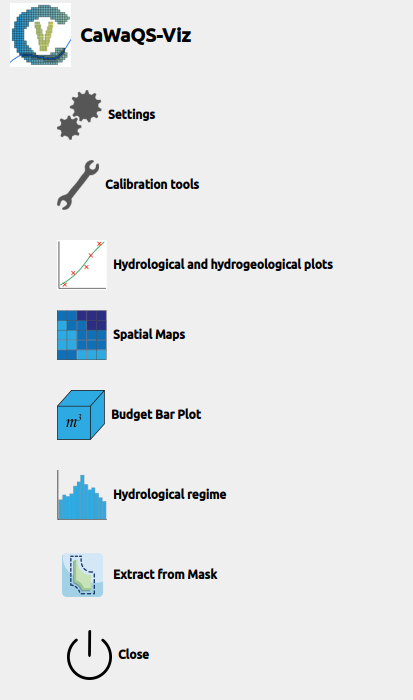
\includegraphics[width=0.4\linewidth]{
        2_application_user_guide/fig/CAWAQS_VIZ_home_page.png
    }
    \caption{Boîte de dialogue d'accueil de l'application \cwv.}
    \label{fig-cwv_home_page}
\end{figure}

L'utilisation de l'extension \cwv~repose sur un projet \script{SIG} préexistant contenant :
\begin{itemize}
    \item les maillages des différents modules de l'application \cawaqs, aux résolutions de sortie de la modélisation ;

    \item des points d'observation et/ou des points d'extraction, situés à l'intérieur des limites de l'emprise du modèle.
\end{itemize}

\subsection{Mode de configuration de \cwv}
\label{sec_config}

Le plug-in doit être configuré pour lire les différents fichiers de sortie de la modélisation et/ou les fichiers d'entrée de \cawaqs~ainsi que les différents maillages. Ce paramétrage du plug-in peut être réalisé dans la fenêtre \gui{Settings}. Pour ce faire, deux procédures sont disponibles \ref{fig-DialogSettings} :
\begin{itemize}
     \item PREMIÈRE FOIS : configurer le projet manuellement dans la seconde partie de la boîte de dialogue (section \ref{sec-auto-detection}).
    \item DÉJÀ CONFIGURÉ : importer un fichier de configuration \script{.json} établi au préalable (section \ref{sec-json_config_project}).

\end{itemize}

\begin{figure}[H]
    \centering
    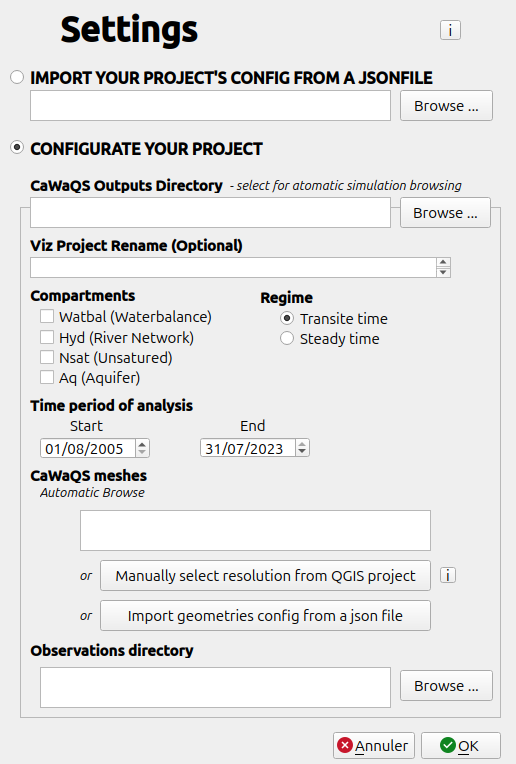
\includegraphics[width=0.45\linewidth]{
        2_application_user_guide/fig/DialogSettings.png
    }
    \caption{La boîte de dialogue \gui{Settings} du plug-in, avec la création d'un nouveau projet sélectionnée.}
    \label{fig-DialogSettings}
\end{figure}

Le détail de ces deux procédures de configuration de l'application est décrit respectivement aux paragraphes \ref{sec-auto-detection} et \ref{sec-json_config_project}.

% ================================================================
% Détection automatique des paramètres du projet à partir du système de fichiers.
% ================================================================

\section{Détection automatique des paramètres du projet}
\label{sec-auto-detection}

Lors de la configuration manuelle d'un projet (plutôt que par import d'un fichier de configuration \script{.json}), \cwv~peut pré-remplir la majeure partie de la boîte de dialogue \gui{Settings} en inspectant le système de fichiers. La seule action requise de l'utilisateur est de parcourir jusqu'au répertoire de sorties \cawaqs~: la détection s'exécute alors automatiquement et renseigne les compartiments, les années de simulation, le régime, le répertoire d'observations et le chemin de configuration des géométries.

La détection est un mécanisme de \emph{meilleur effort}, à visée de commodité. Elle repose entièrement sur les conventions de nommage et d'organisation décrites ci-dessous. Si une convention n'est pas respectée, le champ correspondant est simplement laissé vide et peut être renseigné à la main --- la seule exigence stricte est que le répertoire de sorties contienne au moins un sous-dossier de module reconnaissable (voir \cref{ssec-auto-outcaw}).

La détection s'appuie sur deux sondes indépendantes, ancrées sur deux racines différentes :
\begin{itemize}
    \item le \textbf{répertoire de sorties} \cawaqs~que vous sélectionnez (\cref{ssec-auto-outcaw}) --- pilote les compartiments, les années et le régime ;

    \item le \textbf{fichier de projet QGIS} (\script{.qgz}~/~\script{.qgs}) actuellement ouvert (\cref{ssec-auto-neighbors}) --- pilote la configuration des géométries, le répertoire d'observations et le nom du projet.
\end{itemize}

% ----------------------------------------------------------------
\subsection{Sonde 1 --- depuis le répertoire de sorties \cawaqs}
\label{ssec-auto-outcaw}

Cette sonde est ancrée sur le répertoire de sorties sélectionné via le bouton \gui{Browse}. Elle attend, directement dans ce répertoire, un ou plusieurs sous-dossiers de sortie de module, chacun nommé d'après son module \cawaqs~:

\begin{center}
\begin{tabular}{ll}
    \textbf{Sous-dossier} & \textbf{Compartiment détecté} \\
    \hline
    \script{Output\_AQ}      & \script{AQ} (aquifères)        \\
    \script{Output\_HYD}     & \script{HYD} (réseau hydraulique) \\
    \script{Output\_WATBAL}  & \script{WATBAL} (bilan hydrique de surface) \\
    \script{Output\_NONSAT}  & \script{NSAT} (zone non saturée) \\
\end{tabular}
\end{center}

Au moins un de ces sous-dossiers doit être présent ; sinon la détection échoue et la boîte de dialogue doit être renseignée manuellement.

À l'intérieur de chaque sous-dossier de module, les \textbf{noms des fichiers de résultats binaires} déterminent les années de simulation et le régime. Deux motifs de nommage sont reconnus :

\begin{itemize}
    \item \script{<MODULE>\_<VAR>.YYYYYYYY.bin} --- un pas de temps annuel \textbf{transitoire}. Les huit chiffres encodent deux années consécutives, l'année de début \script{YYYY} suivie de l'année de fin \script{YYYY}, la fin valant le début $+\,1$ (par ex. \script{20102011}). Chaque fichier de ce type contribue par son année de début ; le début le plus ancien et la fin la plus récente définissent la plage de simulation.

    \item \script{<MODULE>\_<VAR>.00.bin} --- un résultat en régime \textbf{permanent}. La présence de ce motif signale une simulation permanente.
\end{itemize}

Le régime est résolu comme suit : \script{Steady} si seuls des noms de fichiers permanents sont trouvés et aucun transitoire ; sinon \script{Transient}. Si les deux motifs coexistent, la simulation est classée \script{Transient} et un avertissement est émis. Si aucune année n'a pu être lue dans un nom de fichier, la plage vaut par défaut \script{1970}--\script{2022}.

L'organisation attendue ressemble donc à ceci :

\begin{lstlisting}[caption={Organisation attendue du répertoire de sorties \cawaqs.},captionpos=b,frame=lines,basicstyle=\ttfamily\footnotesize]
<OUT_CAW>/
|-- Output_AQ/
|     |-- AQ_HEAD.20102011.bin      <-- transitoire (2010->2011)
|     |-- AQ_HEAD.20112012.bin      <-- transitoire (2011->2012)
|     +-- ...
|-- Output_HYD/
|     +-- HYD_Q.20102011.bin
|-- Output_WATBAL/
|     +-- WATBAL_...00.bin          <-- marqueur de regime permanent
+-- Output_NONSAT/
      +-- ...
\end{lstlisting}

\alertinfo{Le régime, la liste des compartiments et les années de simulation sont lus \emph{uniquement} par cette sonde. Parcourir jusqu'au répertoire de sorties est donc l'unique étape obligatoire pour la détection automatique.}

% ----------------------------------------------------------------
\subsection{Sonde 2 --- depuis les voisins du projet QGIS}
\label{ssec-auto-neighbors}

Cette sonde est ancrée sur le fichier de projet QGIS actuellement ouvert (\script{.qgz}~/~\script{.qgs}). Elle relève purement du meilleur effort : chacun des trois éléments ci-dessous est recherché indépendamment, et n'importe lequel peut rester vide sans empêcher la détection.

\begin{itemize}
    \item \textbf{Configuration des géométries} --- la sonde recherche les fichiers correspondant à \script{config\_geometries\_*.json} dans le \emph{même dossier} que le fichier de projet. Si plusieurs correspondent, le plus récemment modifié est retenu.

    \item \textbf{Répertoire d'observations} --- la sonde cherche un dossier nommé \script{DATA\_OBS} au niveau du fichier de projet, puis un niveau au-dessus, puis deux niveaux au-dessus, et s'arrête à la première correspondance.

    \item \textbf{Nom du projet} --- déduit du dossier qui \emph{contient} \script{DATA\_OBS} lorsqu'il est trouvé ; sinon du nom du dossier parent (ou grand-parent) du fichier de projet.
\end{itemize}

Le voisinage attendu du fichier de projet est le suivant :

\begin{lstlisting}[caption={Organisation attendue autour du fichier de projet QGIS.},captionpos=b,frame=lines,basicstyle=\ttfamily\footnotesize]
<project_root>/                     <-- nom utilise comme nom de projet
|-- DATA_OBS/                       <-- repertoire d'observations
+-- <qgis_folder>/
      |-- my_project.qgz            <-- projet QGIS ouvert
      +-- config_geometries_*.json  <-- config des geometries (le plus recent l'emporte)
\end{lstlisting}

\alertwarning{Comme la configuration des géométries n'est recherchée qu'à côté du fichier \script{.qgz}~/~\script{.qgs}, et \script{DATA\_OBS} seulement jusqu'à deux niveaux au-dessus, un projet enregistré en dehors de sa structure de dossiers habituelle laissera ces champs vides. C'est le comportement attendu --- renseignez-les manuellement via le bouton \gui{Configure Geometry} et le champ de parcours des observations.}

% ----------------------------------------------------------------



\section{Configuration du projet à partir d'un fichier \json}
\label{sec-json_config_project}

Une fois un projet configuré (que ce soit par détection automatique ou à la main), sa configuration est écrite sous forme de fichiers \script{.json} dans \script{<OUT\_CAW>/PostProcessing/CONFIG/}, à savoir \script{config\_project\_<name>.json} et \script{config\_geometries\_<name>.json}. Ces fichiers peuvent ensuite être ré-importés directement via la première procédure de configuration, contournant entièrement la détection.

L'import d'un fichier \json~externe peut aussi servir à configurer le projet. Ce fichier est automatiquement enregistré dans le répertoire de post-traitement d'un projet après sa première configuration.

À l'exécution de la boîte de dialogue de paramétrage de l'application \cwv, le sous-répertoire du projet est créé dans le répertoire de post-traitement spécifié. Si le projet n'existe pas encore dans ce répertoire, un sous-répertoire portant le nom du projet est créé, contenant les fichiers de configuration du projet et des résolutions écrits au format \gui{json}.


Ce fichier \json~de configuration de projet est structuré comme suit :

\begin{lstlisting}[language=json]
{
    "json_path_geometries": str,
    "projectName": str,
    "cawOutDirectory": str,
    "startSim": int,
    "endSim": int,
    "obsDirectory": str,
    "ppDirectory": str,
    "regime": str
}
\end{lstlisting}

\vspace{-0.6cm}
Le contenu de chaque objet de ce fichier \json~est le suivant :
\begin{itemize}
    \item \gui{json\_path\_geometries} : chemin absolu du fichier de configuration des résolutions ;

    \item \gui{projectName} : nom du projet ;

    \item \gui{cawOutDirectory} : chemin absolu du répertoire contenant les sorties de modélisation \cawaqs~;

    \item \gui{startSim} et \gui{endSim} : années de début et de fin de simulation au format \script{integer} ;

    \item \gui{obsDirectory} : chemin absolu du répertoire parent contenant les chroniques observées ;

    \item \gui{ppDirectory} : chemin absolu du répertoire de post-traitement. Notez que ce chemin doit déjà exister. Dans le cas contraire, il ne sera pas créé par l'application.

    \item \gui{regime} : régime de modélisation (« Transient » ou « Steady »).
\end{itemize}
